\documentclass[11pt]{article}

% ==== PACKAGES ==== %
% \usepackage{fullpage}
\usepackage{amsmath,amssymb,amsthm}
\usepackage{epic}
\usepackage{eepic}
\usepackage{hyperref}
\usepackage{listings}
\usepackage{float}
\usepackage{graphicx}
\usepackage{fancyhdr}
\usepackage{color}
\usepackage[letterpaper, margin=1in]{geometry}
\usepackage{graphicx}
% ==== MARGINS ==== %
% \pagestyle{empty}
% \setlength{\oddsidemargin}{0in}
% \setlength{\textwidth}{6.8in}
% \setlength{\textheight}{9.5in}

\pagestyle{fancy}
\fancyhf{}
\rhead{CSCI 5622}
\lhead{Homework 1}
\rfoot{Page \thepage}


\newtheorem*{solution*}{Solution}
\newtheorem{lemma}{Lemma}[section]
\newtheorem{theorem}[lemma]{Theorem}
\newtheorem{claim}[lemma]{Claim}
\newtheorem{definition}[lemma]{Definition}
\newtheorem{corollary}[lemma]{Corollary}
\lstset{moredelim=[is][\bfseries]{[*}{*]}}

% ==== DOCUMENT PROPER ==== %
\begin{document}

\thispagestyle{empty}

% --- Header Box --- %
\newlength{\boxlength}\setlength{\boxlength}{\textwidth}
\addtolength{\boxlength}{-4mm}

\begin{center}\framebox{\parbox{\boxlength}{\bf
      Machine Learning \hfill Homework 1\\
      CSCI 5622 Fall 2017 \hfill Due Time Sep 15, 2017\\
      Name: Kumar Bhargav Srinivasan \hfill CU identitykey: kusr7198
}}
\end{center}




\section{K-nearest Neighbor (40pts)}
\textbf{1.2 Analysis}\newline
\textbf{1. What is the role of the number of training instances to accuracy (hint: try different \--limit" and plot accuracy vs. number of training instances)?}\newline
\newline
As the number of training instances increases, \textbf{the accuracy of the solution increases} (Error rate decreases)\newline
Following is the graph which denotes different quantity of train data vs accuracy of the model.\newline
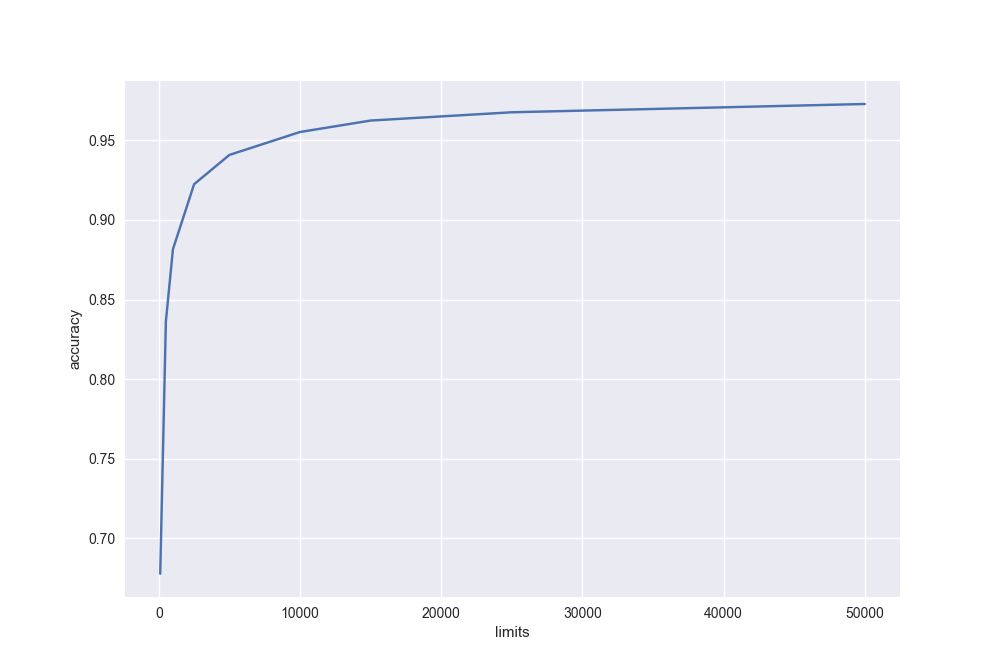
\includegraphics[width=\textwidth]{answer1.png}


\textbf{2. What numbers get confused with each other most easily?}\newline
Following is the observations of the heat map.
\newline Majority 1 : 4 and 9 
\newline Majority 2: 2 and 7
\newline 
\newline\textbf{ 3. What is the role of k to training accuracy?}\newline
\newline In general, As value of k increases above saturation, \textbf{accuracy decreases.}
\newline Below is a graph which shows accuracy vs k values for training data set with 1000 observations, which denotes that if $k >$ 3  then the accuracy decreases drastically.\newline

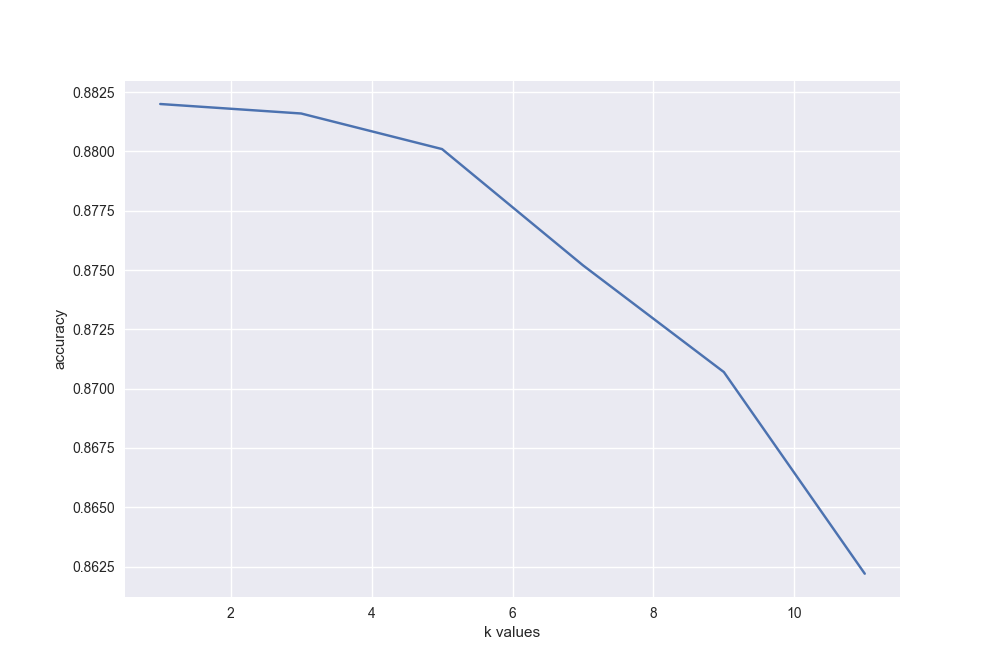
\includegraphics[width=\textwidth]{answer3.png}
\textbf{4. In general, does a small value for k cause overtting or undertting?} \newline
\newline
From the analysis, we could say that K Nearest neighbors  with k=1 implies  to over-fitting, or in most of the cases would lead to over-fitting.\newline
\newline
When k=1 the estimate of the probablity is  based on the closest neighbor,a  single point/sample. This is skews the decisions as there might be sort of distortions like  outliers,mislabelling or noise in data. By higher value of K, decisions made will be robust to distortions.\newline

\section{Cross Validation (30pts)}
\textbf{2.2 Analysis}

\textbf{1. What is the best k chosen from 5-fold cross validation with \--limit 500"?
}\newline best k chosen is 1 with accuracy 86.6 (results attached)
\newline\textbf{2. What is the best k chosen from 5-fold cross validation \--limit 5000"?}
\newline best k chosen was 1 with accuracy of 93.8 (results attached)
\newline best k will be pre-dominantly 3 for higher value of limits
\newline\textbf{3. Is the best k consistent with the best performance k in problem 1?}
\newline No, best k is higher than compared to problem 1 for limited dataset.
\newline For Example : 
for k =3 with 5000 training data Accuracy in problem 1 is 93.1\newline
whereas,
\newline for k =3 with 5000 training data Accuracy in problem 2 is 93.82\newline

\section{Bias-variance tradeoff (20pts)}


Assumptions :\newline
\begin{enumerate}
\item For a given $x,$  $Y(x)=f(x)+ϵ $. 
\item  $Variance(\in) = \sigma_{\in}^2$
\item $E(\in) = 0.$
\item $h_s(x_0) = \sum_{l=1}^{k}y_l $  where $x_{(l)}$ is the l'th nearest neighbor to $x_0$, implies $var(f(x_{l})) = 0$
\item $Err(x_0) = E((y_0 - h_s(x_0)))^2$\newline
\end{enumerate}
 We know from the bias variance tradeoff that $Err(x_0) $ is the following: \newline
$E((y_0 - h_s(x_0)))^2 = bias^2 + variance +  variance(\in) $\newline
 (As derieved by Chenhao Tan in Lecture)\newline
\newline Then the variance of this estimate is:
$variance(h_s(x0)) = var((1/k)*\sum_{l=1}^{k}Y(x_{(l)}))$\newline
$=(1/k^2)*\sum_{l=1}^{k}var(f(x_{(l)})+\in_l)$\newline
$=(1/k^2)*\sum_{l=1}^{k}(var(f(xi))+var(\in_l))$\newline
$=(1/k^2)*\sum_{l=1}^{k}var(\in_l),$ As var$(f(x_{(l)}))=0$\newline 
$=(1/k^2)*(\sigma_\in)^2*\sum_{l=1}^{k}(1)=(1/k^2)*(\sigma_\in)^2 * k ,$ According to assumption that $Var(\in) = \sigma^2$\newline
\textbf{= $(\sigma_\in)^2/k $   -- (a) }\newline 
\newline Bias is equal to difference between actual Target function and predicted  function or hypothesis function which should be close in predicting target values. \newline Target function $Y$ at some value $x_0$ is $f(x_0) + \in_0$\newline
			Square of the bias is as follows : \newline
$bias^2$ = $(Y(x_0)- E_t(f_k(x_0)))^2$ where $E_t$ is estimated target for function.\newline 
=$(Y(x_0)- E_t((1/k)*\sum_{l=1}^{k}(Y(x_l)))^2$\newline
Assuming that $x_{(l)}$ is the l'th nearest neighbor to $x_0$, Expectation can be removed as it becomes actual prediction for $x_l$\newline
=$(Y(x_0)-(1/k)*\sum_{l=1}^{k} Y(x_l))^2$\newline
=$(f(x_0)+\in_0- (1/k) * \sum_{l=1}^{k}f(x_l)+\in_l)^2$ \newline
\newline \textbf{Note : $\in_l$  is added to balance out the bias and the mean over all the values in x will be 0}\newline
 \textbf{$bias^2 = (f(x_0) -(1/k) * \sum_{l=1}^{k}f(x_l))^2    -- (b)$}\newline
\newline Hence from (a), (b) and 2 , \newline 
			$E((y_0 - h_s(x_0)))^2 = bias^2 + variance +  variance(\in) $ becomes, \newline  $E(x_0) = (f(x_0) - (1/k) * \sum_{l=1}^{k}f(x_l))^2$ + $(\sigma_\in)^2/k $ + $\sigma_{\in}^2$




\end{document}
